
%(BEGIN_QUESTION)
% Copyright 2014, Tony R. Kuphaldt, released under the Creative Commons Attribution License (v 1.0)
% This means you may do almost anything with this work of mine, so long as you give me proper credit

If an {\it isolation transformer} (a transformer with the same number of ``turns'' in the primary and secondary coils) is connected between an AC source and an AC load, we will measure the same voltage and the same current at both source and load terminals:

$$\includegraphics[width=15.5cm]{i01253x01.eps}$$

If we calculate power output by the source and power dissipated by the load, the value is the same: 420 Watts ($P = IV$).

\vskip 10pt

Now suppose we analyze a circuit containing a {\it step-up} transformer (one with more turns of wire in the secondary coil than in the primary coil).  With a step-up transformer, the load voltage will be greater than the supply voltage.  In this example, I show a step-up transformer with a 1:2 step ratio:

$$\includegraphics[width=15.5cm]{i01253x02.eps}$$

Assuming the load resistance is completely different from the first (isolation transformer) circuit, what can you deduce about the load current and the power (both source and load) in this circuit?  Is the load current less than the source current?  Is the load current greater than the source current?  Is the load power greater than the source power?  Explain your answers.

\underbar{file i01253}
%(END_QUESTION)





%(BEGIN_ANSWER)

The basic physical law known as {\it The Law of Conservation of Energy} tells us that power cannot come from nowhere, or disappear into nowhere.  If the power source is sending 420 watts into the transformer, then the load must be receiving 420 watts (neglecting any inefficiencies internal to the transformer).  The transformer's step ratio is completely irrelevant as far as {\it power} is concerned!

\vskip 10pt

For a real transformer (with less than 100\% efficiency), the load will receive slightly less than 420 watts of power, the remainder converted into heat at the transformer.

%(END_ANSWER)





%(BEGIN_NOTES)

The only reason I hesitate to tell students they can calculate load current {\it precisely} is because it was not stated whether or not the transformer is ``lossy'' at all.  No real transformer is 100\% lossless, of course, and this is something that we must take into consideration in ``real life.''

I have found that the Conservation of Energy approach not only makes sense to students as they learn to calculate transformer behavior, but it is an excellent reinforcement of a basic physical law, a good understanding of which will serve them well throughout their careers.

%INDEX% Electronics review: transformer ratios

%(END_NOTES)


